\documentclass[11pt]{article}
\usepackage[a4paper,margin=2.8cm]{geometry}
\usepackage{amsfonts}
\usepackage{mathtools}
\usepackage{cancel}
\usepackage{amsthm}
\usepackage{amsmath}
\usepackage{amssymb}
\usepackage{dsfont}
\usepackage[dvipsnames,usenames]{color}
\usepackage[colorlinks=true,linkcolor=NavyBlue,citecolor=NavyBlue,urlcolor=NavyBlue]{hyperref} % for hyperlinks 
\usepackage{floatpag}

% macros 
%%%%%%%%%%%%%%%%%%%%%%%%%%%%%%%%%%%%%%%%%%%%%%%%%%%%%%%%%%%%%%%%%%%%%%%%%%%%
\newcommand{\R}{\mathds {R}}
\newcommand{\red}[1]{\textcolor{WildStrawberry}{#1}} % for color for remarks
\newcommand{\green}[1]{\textcolor{Green}{#1}} % for color for remarks


\title{Fair, Stable Exchange Networks through Quenched Merchant Location and Idiosyncratic Trading Costs}

\author{Nate Dwyer, Sandro Lera, and Alex `Sandy' Pentland}

\begin{document}

\maketitle
\setcounter{section}{0}

\section*{Extended Abstract}

Until not too long ago, people used to live in more self-contained villages,
with local markets where people buy different products.  Take clothing as an
example. Most villages had one or several clothing merchants competing for
customers.  There is some healthy competition among merchants within a village,
as people can flexibly switch according to prices and preferences. But
customers would rarely buy clothing from a faraway village, as the transaction
cost associated with visiting that village would be high,  and could not offset
a marginally better price or quality.  On the other hand, people living far
away from any village are disadvantaged as they always incur such high costs.
Similarly, if there is a specialized product that can only be produced in some
villages, it was harder to find customers across village borders,  making it
more difficult for new products and technologies to succeed. 

From the industrial to the technological revolution, more efficient
distribution channels have emerged, enabling people to buy almost any product
in online stores.  Independent of a customer's physical location, orders can be
delivered to their door within a day.  More specialized products are now sold
globally, and people living far away from hubs benefit from the availability of
a wide range of products.  While such efficiency is beneficial for the economy
as a whole, it comes at the cost of potential monopolies.  Consider a merchant
that manages to sell a product for a few cents cheaper than its competitors. 
Given modern distribution channels, and ignoring potential differences in
quality, every buyer is now incentivized to buy from that one firm at the
cheaper price. One potential outcome is that the competitors follow along,
increase their efficiency, and a new equilibrium is reached.  However, in a
suboptimal scenario, that one firm leverages the temporarily increased revenue
to further outpace and potentially undercut its competitors.  In the short
term, feedback mechanisms kick in, and an initially minor gap in competitive
advantage, mixed with efficient distribution channels, manifests itself in a
monopoly situation. 

We conclude that geographical constraints can lead to unfair and inefficient
conditions for the customers, whereas removal of those constraints can lead to
exploitative monopolies.

In this work, we introduce an individualized tax between buyers and firms based
on distance. Through tuning of this tax and targeted redistribution of tax
money to regions of low economic activity, we show that this model is able to
[put conclusions here, everything else right now is speculation.]

\section{Introduction}
Consider competing firms in a number of small towns. Each town wants to
encourage their local firm to succeed, but at the same time does not want for
its citizens to face monopoly prices. Hence, the towns all levy small,
percentage sales taxes on out of town goods. These taxes increase as the origin
of the good gets more distant.

In addition, the firms that initially do well tend to get better and better
over time and build up an advantage over other firms. This is especially true
with network based firms, where quality of the product is dwarfed by quantity
of the network. 

With enough market power, a profit seeking firm will try to raise barriers to
entry to prevent competition. This stops firms that have new innovations from
surviving long enough to succeed in a market. The distance based tax introduced
in this paper allows start ups to overcome entrenched monopolies' unfair
advantages.

In this paper, we propose a new distance based tax, which we call an
idiosyncratic tax, in order to solve these
problems, then show that it works by modelling an economy that implements the
tax. In section 2 we give an overview of this economy. In section 3 we
formalize the model, and discuss how the firms compete on capacity and price.
In section 4, we discuss results of running the model. In section 5 we expand
the model by allowing for multiple timesteps, and having firms decrease their
costs based on previous profits as a form of investment.
%[change as we add sections]

\section{Economy}
We simulate an economy of buyers and firms in some environment with a distance
metric (e.g. a country, a network economy), then see how firms respond when we
apply the idiosyncratic tax.

\subsection{Geography}
The geography of our model is one-dimensional with periodic boundaries (i.e.
a topological circle) of length $L$. Due to the periodic boundary conditions,
we measure physical distances with the metric $\min(|x-y|, L-|x-y|)$ for any
two points (`agents') $x$,$y$ on the circle. Without loss of generality, we set
$L=1$. Our model does not rely on the implemented geography, and any other,
potentially more realistic topology could be considered.

The left insets of Figure \pageref{fig:fig3x2SingleTimestep} are examples of
such a geography.

\subsection{Buyers}
We randomly place buyers on the circle. Each buyer tries to buy as much product
as possible, but is constrained by a negatively sloped demand curve which
lowers the amount of product they can buy the more expensive the product gets.

\subsection{Firms}
The firms, like the buyers, are also randomly placed on the circle, and compete
non-cooperatively to maximize their profit. In this competition, also known as
a game, each firm makes two choices, first capacity (i.e. how much they
produce), then price. A firm chooses capacity before price because it is
difficult to quickly change capacity due to supply chain restraints, while it
is easier to change a price tag.

\subsection{Idiosyncratic Tax}
The idiosyncratic tax that is introduced by this paper is dependent on a
distance measuere $D$, or ordinal distance, that gives a discrete distance
between every pair of buyers and firms. $D$ is defined such that the closest
firm to a buyer is at ordinal distance $D=1$, the next closest at $D=2$, and
the $n$th closest at $D=n$. Consider a firm and two buyers, one buyer near the
firm, the other distant. The idiosyncratic tax means that the nearer buyer can
buy more cheaply from that firm than can the more distant one. This
incentivizes buyers to purchase from more local firms.

Crucially, this ordinal distance is calculated for every individual type of
product. This means that a dentist and a bakery do not increase each other's
distance from their buyers. In addition, if a firm produces a new product, such
as a drug for a previously incurable disease, it is considered at distance 1
from all buyers, at least until a competitor emerges.

\section{Model Definition}
When firms choose capacity and price, they make their choices in order to
maximize profit. First, the firms compete on capacity, by simultaneously
declaring how much of the product they plan to produce; next, they compete on
price to determine the firms' non-tax prices. This process, consisting of these
two subgames, is called a Kreps-Scheinkman game. The major difference we
introduce to the classical Kreps-Scheinkman game is the idiosyncratic tax,
which significantly alters the pricing subgame.

\subsection{Capacity Game}
The first choice is how much capacity $\hat q_i$ each firm $i$ wishes to
install. The firm's desire to increase capacity is limited by two factors.
First, firm $i$ incurs a unit price of $c_i$ for every unit of product they
install, regardless of whether or not the product is sold. Second, because the
buyers have a limited demand, eventually the buyers will stop buying.

The capacity subgame acts much like a Cournot game.\footnote{A Cournot game is
where firms compete only on quantity, and sell all of the quantity at the
market clearing price.} The difference is that instead of being assigned a
market clearing price and selling everything they produce, in our model the
firms compete on price in a second subgame where they choose a price. Only
after that do the buyers determine how much of each firms capacity is sold.

\subsection{Pricing Game}
Each firm $i$, having chosen a capacity $\hat q_i$, now chooses a price, $p_i$.
Consider two vending machines right beside one another selling the same soda,
with one machine selling soda at a cheaper price than the other. In this
subgame, buyers will use the cheaper machine first, but if the buyers demand
more soda than that machine's capacity, buyers will switch to the more
expensive machine when the cheaper one runs out of soda. Competition on price
in such a manner is called an Edgeworth game. Edgeworth games are very
difficult to find an equilibrium in, as depending on demand and capacity, a
variety of strategies can be employed.

By choosing a lower price, a firm can undercut competitors, ensuring that
buyers choose to buy from them instead of other firms. Since the amount a buyer
purchases increases as the product gets less expensive, a lower price increases
the amount of product purchased in total. But the capacity limitation on total
quantity sold by a firm means that a single firm usually can't sell to the
entire market, and it could be more profitable to just sell a low quantity at a much higher price.

\subsection{Idiosyncratic Tax}
The idiosyncratic tax is designed to promote buyers purchasing locally by
imposing no tax if a buyer purchases from the nearest firm, and then increasing
the tax in discrete steps as firms get more and more ordinally distant. Since
each buyer-seller pair can have a different tax, the tax can cause two buyers
to perceive separate prices at the same firm.

For any buyer $b$ and firm $i$, we define the ordinal distance $D = D(b,i)$
such that the firm $i$ that is physically closest to $b$ has distance
$D(b,i)=1$, the next closest has distance $D=2$, and the $n$th closest has
distance $D=n$.  Thus, if buyer $b$ buys from firm $i$, the total price,
including tax, is given by $p(b,i) = p_i + p_i \cdot r(D(b,i)^\gamma -1)$
where $\gamma$ is the coefficient governing how quickly the tax increases, and
$r$ is a simple scaling coefficient.

Implementing this tax gives the buyers individualized preferences
over the firms. For example, imagine two firms $i$ and $j$, and let $p_i <
p_j$. Without any tax, every buyer prefers buying from $i$ versus buying from
$j$. But with the tax, this could change. Say that buyer $b$ is very close to
firm $j$, and very far from firm $i$, which would mean that $D(b,i) \gg
D(b,j)$. Then buyer $b$ would prefer to buy from $j$ despite $j$'s price
being higher because $p_i + p_i\cdot r(D(b,i)^\gamma - 1) > p_j + p_j\cdot
r(D(b,j)^\gamma -1)$. 

This gives rise to two interesting limit cases, one where $\gamma = 0$, and the
other where $\gamma = \infty$. When $\gamma = 0$, no firms are taxed anywhere,
so the game simplifies into a pure Kreps-Scheinkman game. In contrast, when
$\gamma = \infty$, it becomes impossible for buyers to purchase from non local
firms, and so the firms all impose monopolistic prices.

\subsection{Buyer Behavior and Rationing}
After the firms have finished determining capacity and price, and the
idiosyncratic tax has been incorporated into the prices, the buyers conduct
purchases as follows.

Let the set of buyers be called $B$. Each buyer $b\in B$ buys a quantity $q_b =
\sum_{i\in S} q_{b,i}$, where $q_{b,i}$ is the amount buyer $b$ buys from the
firm $i$. The buyer's all have identical demand curves $p_\text{max} + q_b =
a$, where $a$ is the endowment they are given exogenously, and $p_\text{max}$
is the maximum price they pay (including tax). Each buyer tries to maximize
$q_b$ while keeping $P + Q \le a$. In other words, they buy from the cheapest
available firm until they hit the demand curve.

If a buyer perceives multiple firms as offering identical prices, they buy from
all such firms in identical amounts until either the buyer hits their demand
curve, or a seller runs out of capacity. 

\subsection{Profit Function}
Finally, firm $i$, having chosen quantity $\hat q_i$ and price $p_i$, and
having sold the product to buyers, will earn a profit:

\begin{equation}
    \Pi_i = p_i\sum_{b\in B} q_{b,i} - c_i\hat q_i.
\end{equation}

Note that while the firm can choose both their capacity $\hat q_i$ and their
price $p_i$, their cost per unit $c_i$ is set exogenously. Also, each $q_{b,i}$
is chosen by the buyer $b$ so that they buy as much as possible while staying
under their demand curve $P+Q\leq a$; this is where taxes affect the firm's
profit.

If the firm sells all of their capacity, then $q_i = \hat q_i$, and the profit
equation simplifies to:
\begin{equation}
    \Pi_i = (p_i- c_i)\hat q_i,
\end{equation}
which is the net profit per unit multiplied by quantity sold.

\subsection{Numerical Approximation}
Because the buyers have individualized preferences and the pricing game does
not necessarily have a `best' strategy, it is difficult to determine a
generalized, theoretical solution to the model laid out above. Instead, we
numerically determine the Nash equilibrium.\footnote{A Nash equilibrium
for a game is a set of choices, one for each player, such that upon seeing the
other firm's choices, could increase their payoff by changing strategies. In
our model, the players are firms, the payoff is profit, and the choices are
either capacity or price, depending on the subgame.}

To find the capacities and prices that the firms will choose, we begin by
discretizing the capacity and pricing choices so we only have a finite number
of possible combinations. Then, for every outcome of the capacity game, we find
the Nash equilibrium of the pricing game using the Python library Gambit. Then,
using the equilibrium prices, we calculate the profits for every outcome of the
capacity game. We finally use this information to find the Nash equilibrium of
the capacity game, again using Gambit.

\section{Examples}
Figure \ref{fig:fig3x2SingleTimestep} contains the output of five instances
of finding the numerical solution for different $\gamma$ and costs. In the
first two rows $\gamma=0$, with the one difference being that in Row 1, both
Firm 1 and Firm 2 have the same cost, and in Row 2, Firm 1 has a 1\% lower cost
than Firm 2. In Row 1, the firms sell the same amount of product and make the
same amount of profit. But in Row 2, Firm 1 sells 33\% more quantity and makes
53\% more profit. As a side note, since when $\gamma = 0$ there is no tax on
distance, we can see on the left insets of these rows that buyers do not
necessarily buy from the closest firm.

In the Rows 3, 4, and 5, we let $\gamma = .5$ instead. In Row 3 we can see a
mirror of Row 1, where both firms, faced with the same costs, produce the same
quantity, and make the same profit. But in row 4, where we give Firm 1 the same
advantage we game them in the row 2, they sell the same amount, and only make
12\% more profit than Firm 2. To increase their market share, Firm 1 needs to
reduce their costs to 80\% of Firm 2, as shown in row 5.

The idiosyncratic tax thus acts as a dampener, preventing companies with
slight advantages from acquiring overwhelming market dominance, while still
ensuring that minor innovations are profitable. But, if one firm is
significantly better, as in Row 5, then that firm will still dominate the
market.

\begin{figure}[[p!htb] % p stands for 'entire page', '!htb' is to insert as close to code as possible
  \floatpagestyle{empty} % remove page number
  \centering
  \vspace{-2cm} % shift upwards to get more space for caption
  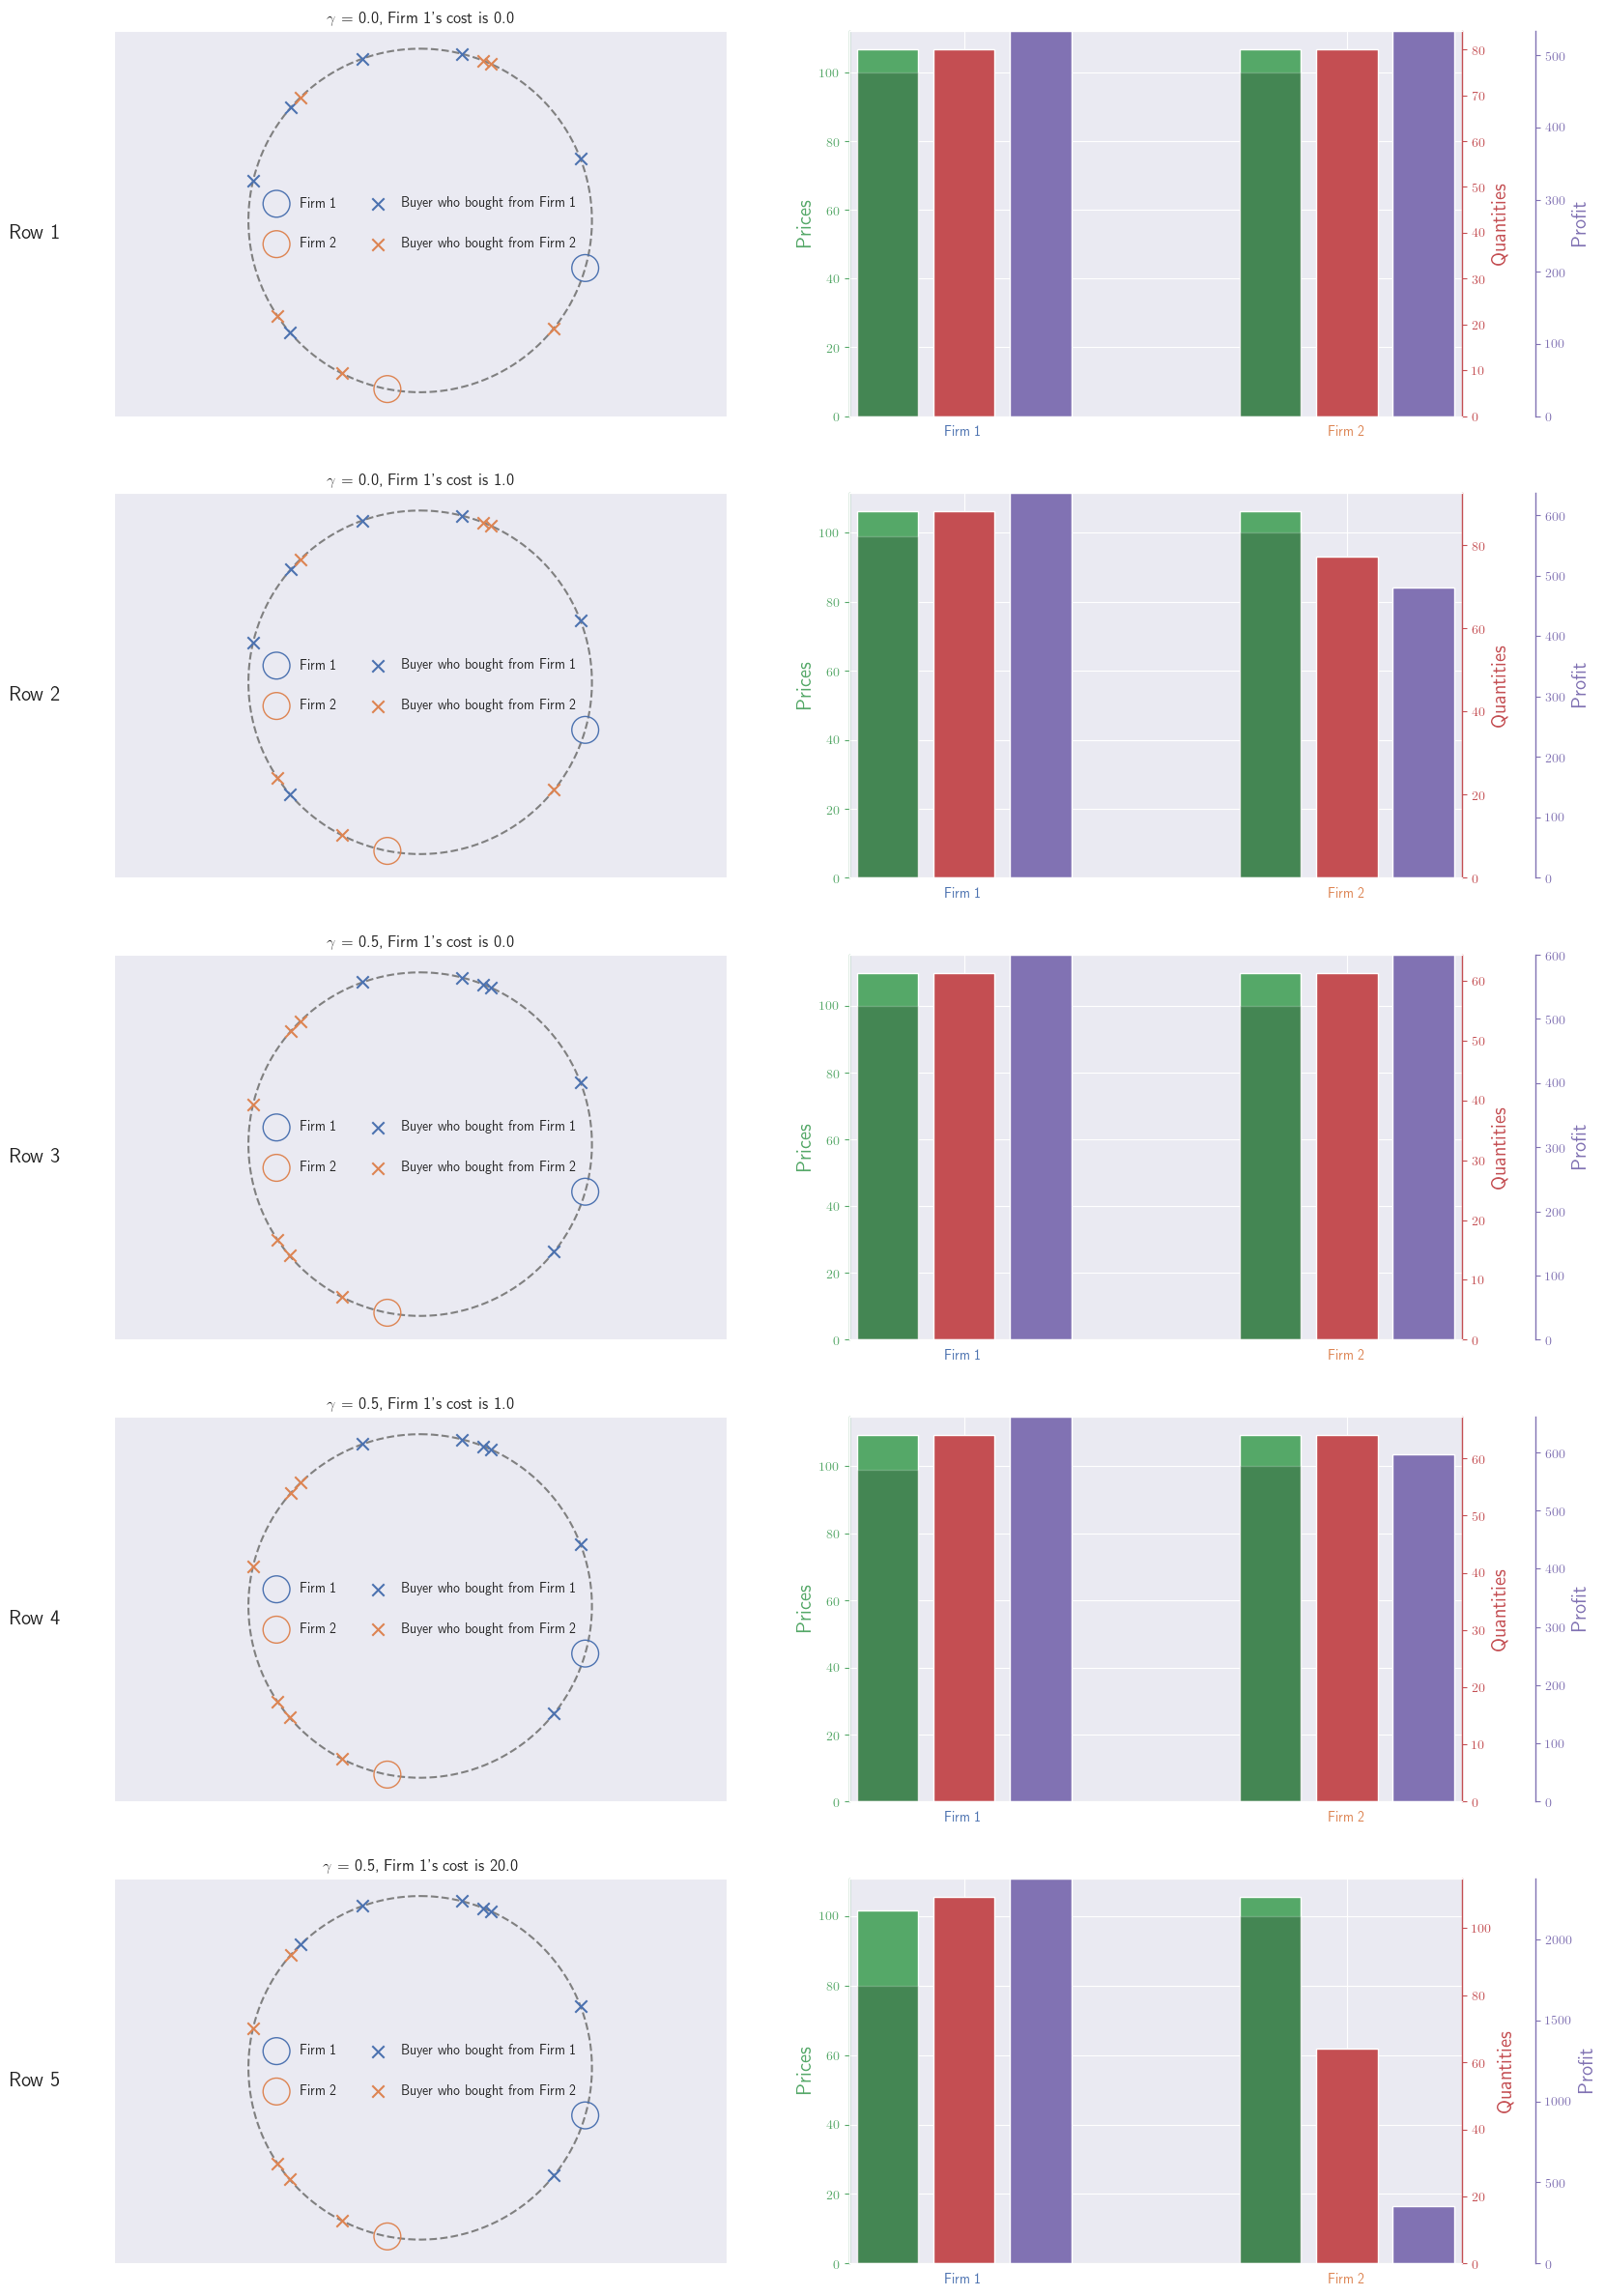
\includegraphics[width=\linewidth]{5x2plot.png}
  \caption{\small{Above are the model's results for a variety of
  conditions. The Rows 1 and 2 have $\gamma=0$, while Rows 3, 4, and 5 have
  $\gamma = .5$. In Rows 1 and 3, the firms have an equal cost per unit, sell
  equal quantity, and make equal profit. In Row 2, where $\gamma=0$, a 1\%
  difference in cost means Firm 1 has a 10\% greater market share, and a 53\%
  larger profit.
  In Row 4, where $\gamma=.5$, Firm 1's 1\% difference in cost now results in
  an equal market share, but they still profit 12\% more. To get a larger
  market share, as in Row 5, Firm 1 must have a 20\% lower cost per unit. This
  means that $\gamma$ acts as a dampener on monopolization by increasing the
  amount of innovation needed to gain market power while still encouraging
  innovation. %[Check numbers after new gamma]
  }}
  \label{fig:fig3x2SingleTimestep}
\end{figure}

\section{Dynamics}
We run this model once for every timestep, then update the costs for the firms
between the timesteps. Every timestep we determine which firm has made the most
profit. For that firm, we reduce its cost per unit by 5\% in order to simulate
the company investing its excess profits in itself to become more profitable in
the long term. 

\end{document}